\documentclass{article}
\usepackage[T1]{fontenc}
\usepackage[utf8]{inputenc}

\usepackage{cmbright}
\usepackage[T1]{fontenc}

\usepackage{multicol}

\usepackage{amsmath}
\usepackage{amsfonts}
\usepackage{amssymb}
\usepackage{tikz}
\usepackage{graphicx}
\graphicspath{  {./images/} }
\setlength{\parindent}{0pt}
\usepackage{changepage}
\usepackage{verbatim}
\usepackage{physics}
\usepackage{derivative}
\usepackage{bm}
\usepackage[colorlinks=true, linkcolor=blue, urlcolor=blue, citecolor=blue, anchorcolor=blue]{hyperref}

\addtolength{\oddsidemargin}{-.25in}
\addtolength{\textwidth}{0.5in}

\makeatletter
\newcommand*\bigcdot{\mathpalette\bigcdot@{.5}}
\newcommand*\bigcdot@[2]{\mathbin{\vcenter{\hbox{\scalebox{#2}{$\m@th#1\bullet$}}}}}
\makeatother

\DeclareMathOperator{\di}{d\!}
\newcommand*\Eval[3]{\left.#1\right\rvert_{#2}^{#3}}

\newcommand{\uvec}[1]{\boldsymbol{\hat{\textbf{#1}}}}
\newcommand{\vr}[1]{\textbf{#1}}

\newcommand{\thus}[0]{\; \; \longrightarrow \; \;}

\newcommand{\lag}{\mathcal{L}}
\newcommand{\ham}{\mathcal{H}}

\title{Distance Estimation Simulations}
\author{Ryan Liu}
\date{Last updated: May 30, 2021}

\begin{document}

\maketitle

\section{Resources Used}

\section{Results}

Larger black hole mergers produce gravitational waves with a greater amplitude; therefore, it would be expected that there is a positive correlation between black hole mass and the maximum distance of observation at any given SNR threshold. However, larger black holes also have slower orbits, and therefore produce waves of lower frequency (i.e. shorter duration), which has a negative impact on the strength of the signal. \\

From Figure \ref{fig:mass}, we see that at low masses, the increase in signal amplitude is more significant than the decrease in signal time. However, at approximately 60 $M_\odot$, the tradeoff becomes relatively balanced. This suggests that the black holes easiest to detect will have masses around 55 to 70 $M_\odot$. 

\begin{figure}[!htb]
    \center{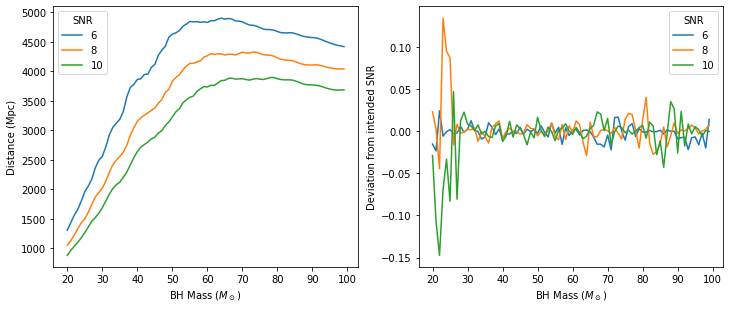
\includegraphics[width=\textwidth]{SNR18.png}}
    \caption{\label{fig:mass} (Left) Maximum distance of observation at different SNR thresholds for aLIGO design sensitivity; (Right) Deviation of parameter estimation from desired SNR}
\end{figure}

We see from Figure \ref{fig:multipledistance} that the same trends are observed at A+ design sensitivity; however, for Cosmic Explorer, there appears to be a linear, negative correlation between black hole mass and maximum distance of observation. The distance threshold for Cosmic Explorer is above 10 Gpc, corresponding to a redshift of over 10 -- therefore, small decreases in wave frequency can lead to very large decreases in signal time. \\

\begin{figure}[!htb]
    \center{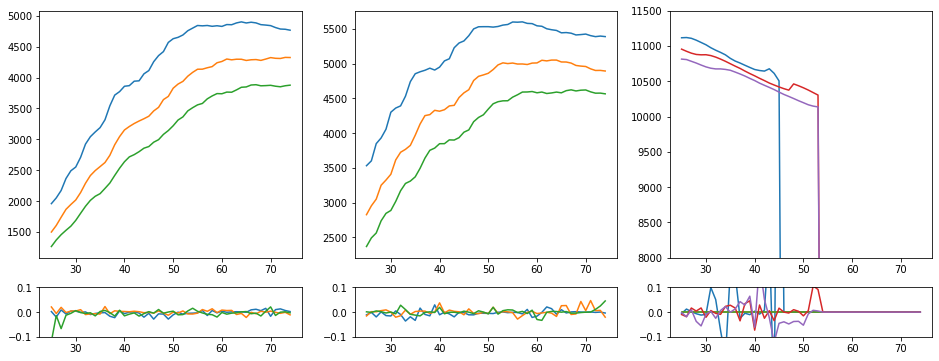
\includegraphics[width=\textwidth]{SNR19.png}}
    \caption{\label{fig:multipledistance} (Top) Maximum distance of observation at a SNR threshold of 6, 8, and 10 for aLIGO design sensitivity, A+ design sensitivity, and Cosmic Explorer design sensitivity; (Bottom) Deviation of parameter estimation from desired SNR}
\end{figure}

Two immediate problems surfaced when attempting to determine the distance threshold for the Cosmic Explorer PSD -- the parameter estimation function failed to accurately converge onto the desired SNR, with deviations often approaching $\pm 1$; furthermore, above a certain black hole mass, wave frequencies were so low that with the extreme redshift, the entire waveform was below the low frequency threshold. 



\section{Issues in Function Accuracy}

To determine why the distance estimation function failed in execution for large black hole mergers using the Cosmic Explorer PSD, we calculate the expectation SNR for mergers of different masses and different distances. From Figure \ref{fig:maxdistance}, we see that starting around 9 Gpc, entire waveforms fall below the low frequency cutoff, and therefore have an undefined SNR. However, especially for large-mass mergers, at marginally smaller distances the SNR is still very high ($\sim 10^1$). Therefore, for mergers that create an error in the distance estimation function, we can approximate the maximum distance to simply be the maximum distance at which a signal exists above the threshold low frequency. \\  

\begin{figure}[!htb]
    \center{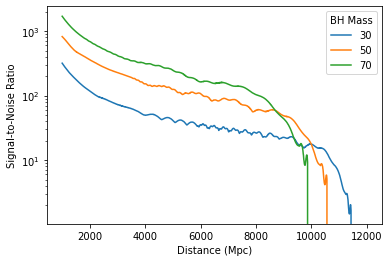
\includegraphics[width=3in]{SNR20.png}}
    \caption{\label{fig:maxdistance} Expectation SNR for equal-mass BH mergers with Cosmic Explorer design sensitivity at various distances}
\end{figure}

Additionally, it can be seen in Figure \ref{fig:maxdistance} that although the expectation SNR exhibits an overall downwards trend as expected, the value appears to oscillate with a small amplitude -- the period and amplitude of oscillation appears to be larger for higher-mass mergers as well. Looking closely at a small segment of the distance-SNR curve, we see that this ``oscillatory" nature is very well defined; furthermore, there appears to be random variation in the expectation SNR as well. \\

There does not appear to be a clear explanation for this phenomenon, but the non-smooth SNR-distance curve is possibly a relic of the generation of waveforms -- due to the low frequency threshold, the SNR will suddenly drop every time the increased redshift leads to the discarding of one oscillation. 


\begin{figure}[!htb]
    \center{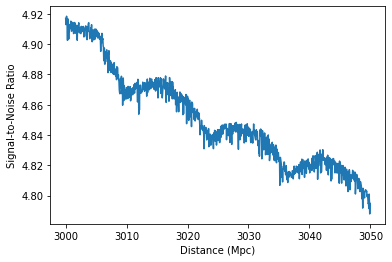
\includegraphics[width=3in]{SNR21.png}}
    \caption{\label{fig:label} Expectation SNR of a 30 $M_\odot$ black hole merger at aLIGO design sensitivity; the distance resolution is $0.05$ Mpc}
\end{figure}

\end{document}